\documentclass[a4paper,10pt]{article}

\usepackage{ucs}
\usepackage[utf8x]{inputenc}
\usepackage{amsmath}
\usepackage{amssymb}
\usepackage{subfigure}
\usepackage{fontenc}
\usepackage{graphicx}
\usepackage{capt-of}
\usepackage{natbib}
\bibliographystyle{apj.bst}
\usepackage{aas_macros}

\usepackage[dvips]{hyperref}

\date{03/15/15}

\begin{document}
 \section{Introduction}
 --Initial Problem (graph of obs data)\\
 --First thoughts (Hypothesis)\\
 \subsection{magnitude cut}
 Explanation for magnitude cut \label{magnitudecut}
 \section{Method}
 
 I set up a 3 dimensional grid in stellar distance (r) mass (M) and age (t). The range 
 of these three variables can be easily adjusted, as can the binning. In accordance to the observational data I attempt to model, 
 distance ranges from 0 to $r_{max}=3kpc$ and mass ranges
 from $M_{min}=5M_\odot$ to $M_{max}=50M_\odot$. The mass-distribution will follow the Salpeter Initial Mass Function (IMF)
 \citep[see][]{1955ApJ...121..161S}. Because the IMF follows an inverse power law, I use a logarithmic mass-grid.\\ 
 
 For age I use a single axis for all stars ranging from 0 to the main sequence age of the least massive star ($t_{ms}(M_{min})$). 
 Because in first order the main sequence age ($t_{ms}$) of 
 a star is a strictly monotonic increasing function of M one can set: $t_{ms}(M_{min})=t_{max}$. With $M_{min}=5M_\odot$ this 
 translates to $t_{max}\approx 104Myr$. The age axis is defined logarithmic to make sure massive stars with small $t_{ms}$ are correctly
 represented. \textbf{Another possibility would have been to use a separate age-axis for every star ranging from 0 to $t_{ms}(M)$}. \\ 
  
 The information I have about any given star is its mass, its age and its distance from earth. From this information
 I derive its fractional main sequence age ($\tau$), its apparent magnitude (V) and \textbf{ultimately the probability density for all stars}.\\  
 
 The first step is to use analytical formulations derived from a stellar evolution model by \citet*{2000MNRAS.315..543H} which approximates the
 stellar evolution as a function of initial mass ($M_{ini}$), fractional main sequence age ($\tau$) and metalicity (Z).
 To do this, I need to find $\tau$. Using equation 5 of \citep{2000MNRAS.315..543H} \textbf{give equation?} I know the main sequence age 
 $t_{ms}(M)$ and $\tau$ then becomes: $\tau(M)=\frac{t}{t_{ms}(M)}$. \textbf{Since I only include stars on the main sequence, I can safely include
 the condition: $\tau<1$ to cut down on computing time.}
 I then use Equation 12 and 13 from the same paper to compute luminosity and radius for a star on the main sequence\footnote{
 \citet{2000MNRAS.315..543H} cites \citet*{1996MNRAS.281..257T} for Zero Age Mainsequence (ZAMS) Radii and Luminosities. 
 In Equation 1 of the cited paper there is a typo, where: $\gamma + M^3$ has to be $\gamma \cdot M^3$.}.\\
 
  \begin{figure}[h!]
  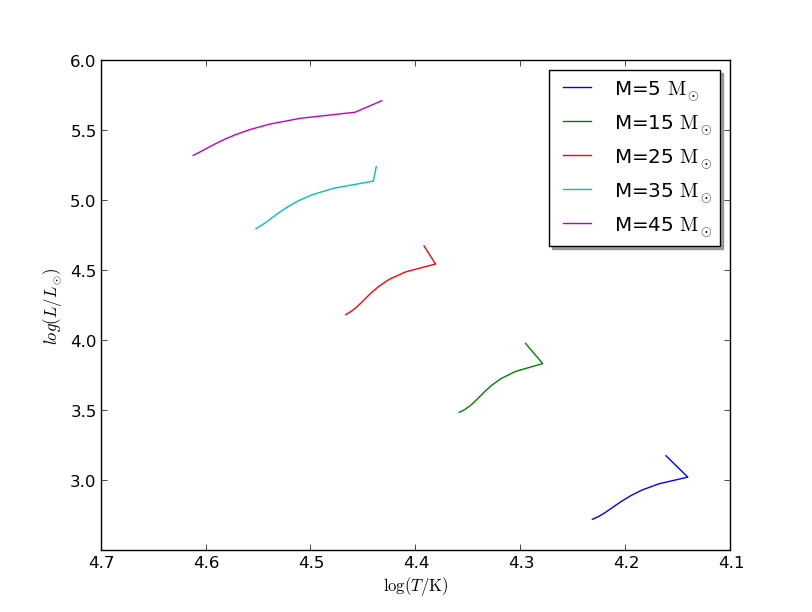
\includegraphics[width=\textwidth]{lumiradius}
  \caption{HRD for five different stars on their main sequence based on the evolutionary model of \citet{2000MNRAS.315..543H} \label{lumiradius}}
 \end{figure}
 
 For my purposes I use Z=0.02 for all stars to simulate a metalicity similar to that of our sun according to \citet*{1998SSRv...85..161G}\\
 \textbf{I now run this model for every possible mass-age combination and save the results in a matrix. This way I don't have to call the program for
 every distance-mass-age combination and massively cut down on computing time.}\\
 Using known distance, mass, age, fractional main sequence age, luminosity and radius for any given star I can  
 compute the apparent magnitudes. I use the following equations:
 
 \begin{equation}
  M_{V}=V-5\cdot\log(r)+5-A(r)
  \label{MV}
 \end{equation}
 
 \begin{equation}
  M_{bol}=M_{V}+BC
  \label{Mbol}
 \end{equation}
 
 \begin{equation}
  \log(L/L_\odot)=0.4\cdot(4.72-M_{bol})
  \label{LMbol}
 \end{equation}
 
 Where $M_{V}$ is the absolute visual magnitude, $\log(r)$ is the logarithm to base ten of the distance from earth. A(r) is the reddening,
 $M_{bol}$ is the absolute bolometric magnitude and BC is the Bolometric Correction. Using equations \ref{MV}, \ref{Mbol} and \ref{LMbol}
 I can compute the apparent visual magnitude V:
 
 \begin{equation}
  V=5\cdot\log(r)-5+A(r)+4.72-\frac{\log(L/L_\odot)}{0.4}-BC.
 \end{equation}
 
 To get a rough approximation for reddening, I use \citet*[Figure 9]{2005AJ....130..659A}. I linearly interpolate the three intervals between:
 distance=0kpc, A=0; distance=1kpc, A=0.9; distance=2kpc, A=2.25 and distance=3kpc, A=3.273.\\
 The next thing I need to know are the probability densities for stars in space $\left(\frac{dp}{dV}\right)$, mass 
 $\left(\frac{dp}{dm}\right)$ and age $\left(\frac{dp}{dt}\right)$. In my simulation I assume a homogenous density of stars. \textbf{(is this 
 misleading? Because density does not have to be in space)} Because of
 the radial symmetry of the problem, the distribution is solely dependant on the distance from earth,
 
 \begin{equation}
  \frac{dp}{dV}=\frac{1}{V_{tot}}=\frac{1}{\frac43\cdot\pi\cdot r_{max}^3}.
  \label{dpdV}
 \end{equation}
 
 I assume a constant star formation rate, so the probability density in age is $\frac{dp}{dt}=\frac{1}{t_{ms}}$. I do however 
 use a logarithmic binning in age. Thus I can not use $\frac{dp}{dt}$ but instead need to find $\frac{dp}{d\log t}$ using the following 
 relation $d\log t=\frac{dt}{t \ln 10}$; 

 \begin{equation}
  \frac{dp}{d\log t}=\frac{t\ln 10}{t_{ms}}.
 \end{equation}
 
 I assume the stars are distributed in mass following the Salpeter Initial Mass Function (IMF):
 $\frac{dp}{dM}=A\cdot M^{-2.35}$ \citep*{1955ApJ...121..161S}. Similar
 to the density function in age, I need to convert it to a logarithmic binning using $d\log M = \frac{dM}{M\ln 10}$
 
 \begin{equation}
  \frac{dp}{d\log M}=\ln 10 \cdot A\cdot M^{-1.35},
 \end{equation}
 
 Where A is a normalization factor, that follows from: 
 
 \begin{equation}
  1=\int_{M_{min}}^{M_{max}}A\cdot M^{-2.35} dM =\left[ -1.35\cdot A\cdot M^{-1.35}\right]_{M_{min}}^{M_{max}},
 \end{equation}
 
 \begin{equation}
  A= \frac{1.35}{M_{min}^{-1.35}-M_{max}^{-1.35}}.
 \end{equation}
 
 With this information I can formulate the overall probability density function for the stars in my sample with regard to $\tau$
 
 \begin{equation}
  \frac{dp}{d\tau}=\frac{dp}{dV}dV \cdot \frac{dp}{d\log t}d\log t \cdot \frac{dp}{d\log M}d\log M\cdot \frac{1}{d\tau}
 \end{equation}
 
 I will only consider stars with $\tau\le 1$ and $V\le 9$ This way I count every
 star on the main sequence, that falls below my magnitude cut (see \ref{magnitudecut}). 
 
 \newpage
 \section{Tests}
 I conducted a few consistency and numerical tests to see, whether my program produces formally correct results. 
 The most prominent I will explain in detail:
 
 \begin{figure}[h!]
  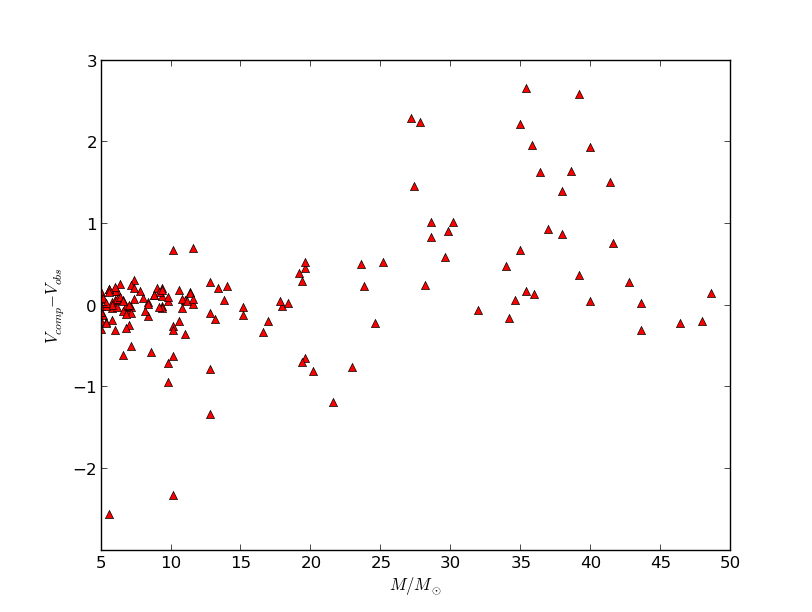
\includegraphics[width=0.9\textwidth]{diffmagmass}
  \caption{Difference between computed and observed magnitudes as a function of mass\label{diffmagmass}}
 \end{figure}
 
 
 The theoretical magnitudes ($V_{comp}$) were computed using stellar radius, luminosity and distance. The observational magnitudes ($V_{obs}$)
 were taken from a sample of 150 stars between M=5M$_\odot$ and M=48M$_\odot$ from \citep{2014A&A...570L..13C}
 
 Figure \ref{diffmagmass} shows the difference between computed and observed magnitudes as a function of mass. There is a significant
 deviation towards higher $V_{comp}$ at high masses. This can be explained using Figure \ref{castroetal}:
 \begin{figure}
  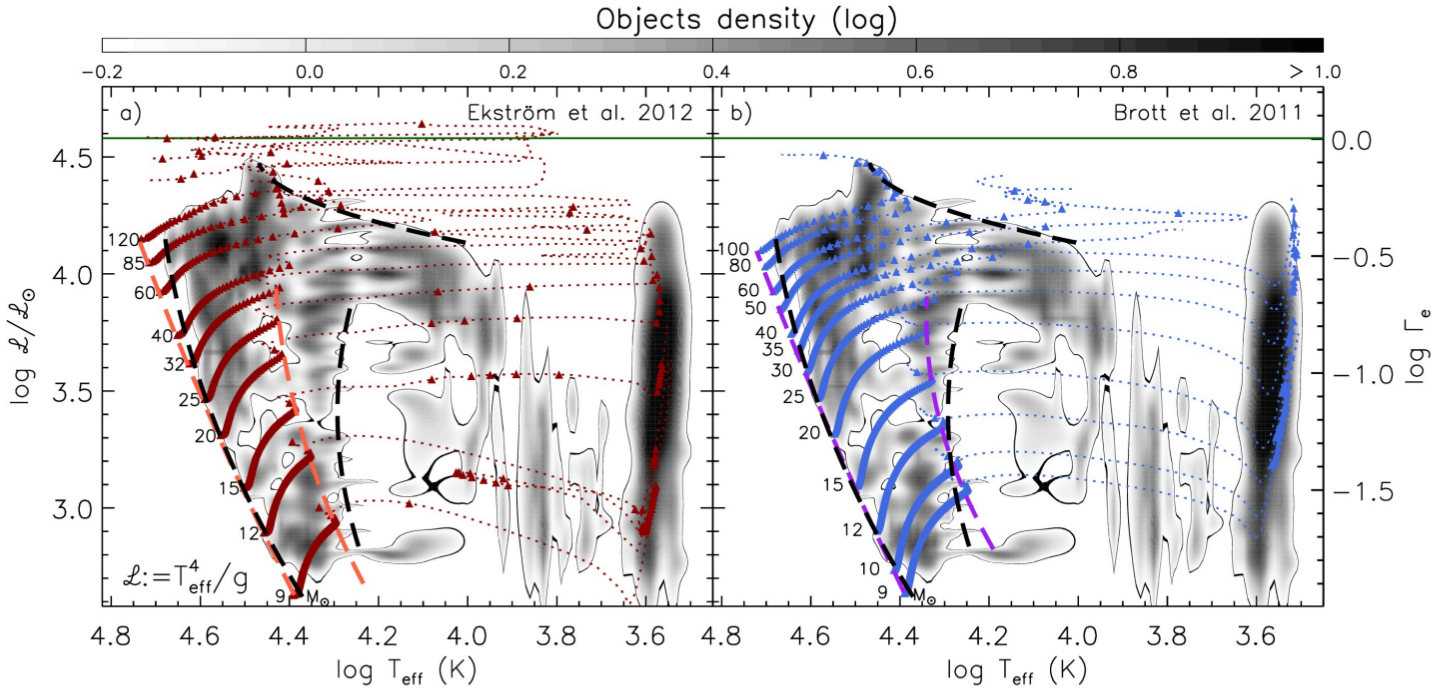
\includegraphics[width=\textwidth]{Castroetal}
  \caption{Grey scale representation of the probability density distribution of the location of 575 Galactic stars in the sHRD.
  Overlayed are stellar evolution tracks for non-rotating stars with solar composition a)\citet{2012A&A...537A.146E}
  and b)\citet{2011yCat..35309115B}. The ZAMS and TAMS positions of the models are connected through orange and purple dashed lines.
  Red and blue triangles are placed on the tracks separated by 0.1 Myr \citep{2014A&A...570L..13C}\label{castroetal}}
 \end{figure}

 My code uses an evolutionary model similar to model a). $V_{obs}$ however is obtained using a model similar to model b).
 Model b) accounts for convective overshooting to a higher degree and thus the lifetime of stars is expanded. This would account for
 minor deviations. Because of the difference in position of TAMS in the HRD, \textbf{I STILL DON'T GET IT}.
 The massive deviations between $M=25M_\odot$ and $M\approx 43M_\odot$ can be explained by taking into account inflation. 
 Near TAMS on the main sequence massive stars will undergo an expansion of their envelopes. This gives rise to a big shift on the
 HRD.
 
 \begin{figure}[h!]
  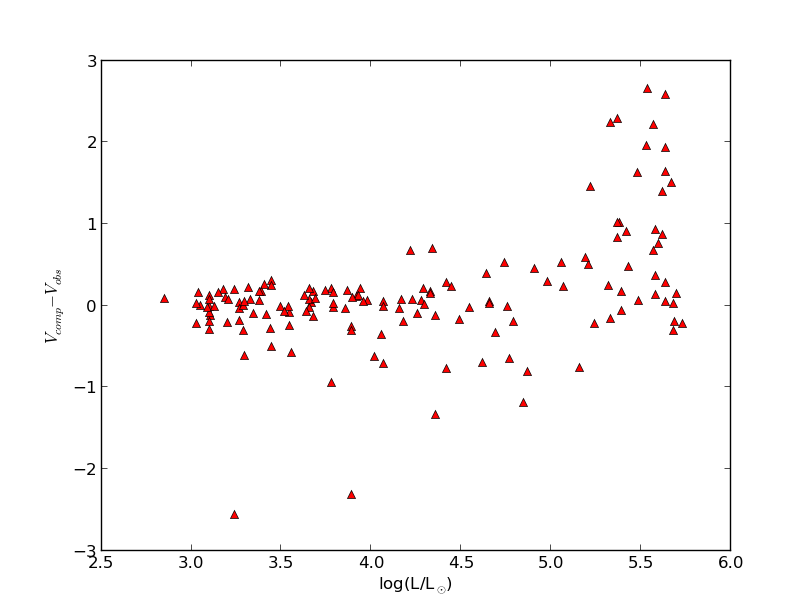
\includegraphics[width=0.9\textwidth]{diffmaglogL}
  \caption{Difference between computed and observed magnitudes as a function of $\log(L/L_\odot)$}
 \end{figure}
 
 \begin{figure}[h!]
  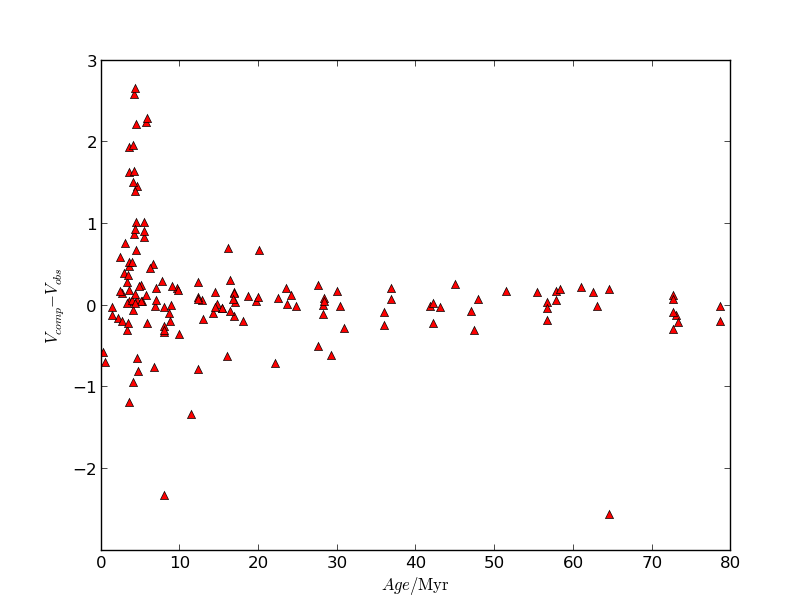
\includegraphics[width=0.9\textwidth]{diffmagAge}
  \caption{Difference between computed and observed magnitudes as a function of fractional main sequence age $t_{ms}$}
 \end{figure}
 
 \begin{figure}[h!]
  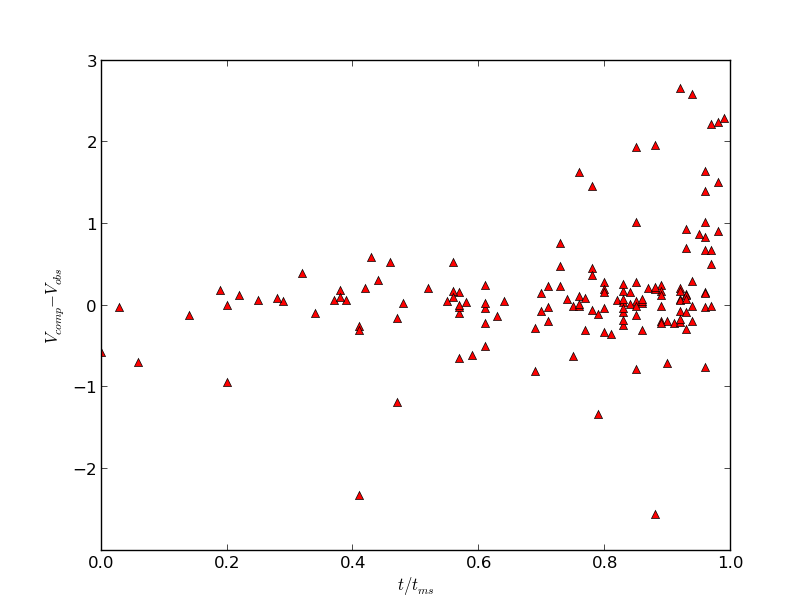
\includegraphics[width=0.9\textwidth]{diffmagfracms}
  \caption{Difference between computed and observed magnitudes as a function of age}
 \end{figure}
 
 
 
 The deviation to negative values is mostly caused by extinction. It is most prevalent in lower absolute ages. 
 Stars of lower ages are primarily found in regions of active star formation. This would mean, that they are found in regions
 of high gas density. This gas will cause extinction and thus increase $V_{obs}$. My model for extinction does not take into account 
 these density fluctuations.
 
 
 \begin{figure}[h!]
  \begin{minipage}{0.49\textwidth}
   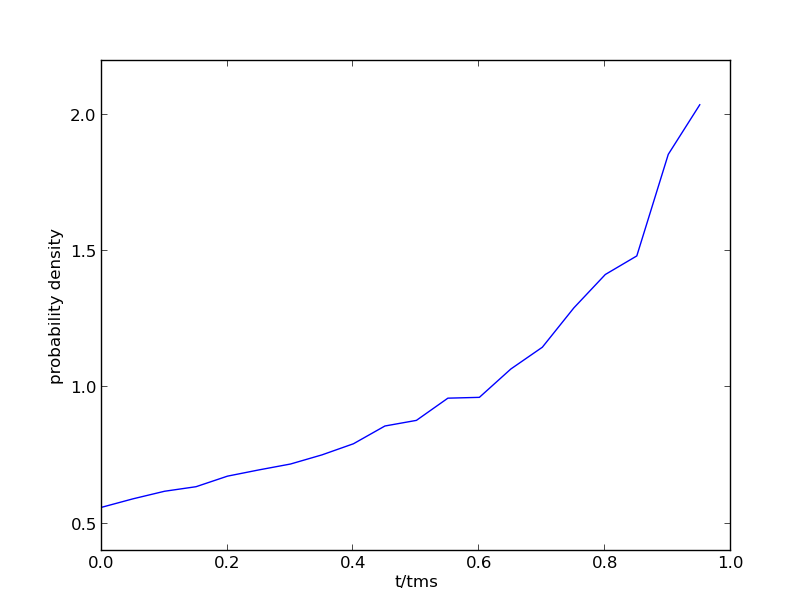
\includegraphics[width=\textwidth]{100-100-100}
  \end{minipage}
  \begin{minipage}{0.49\textwidth}
   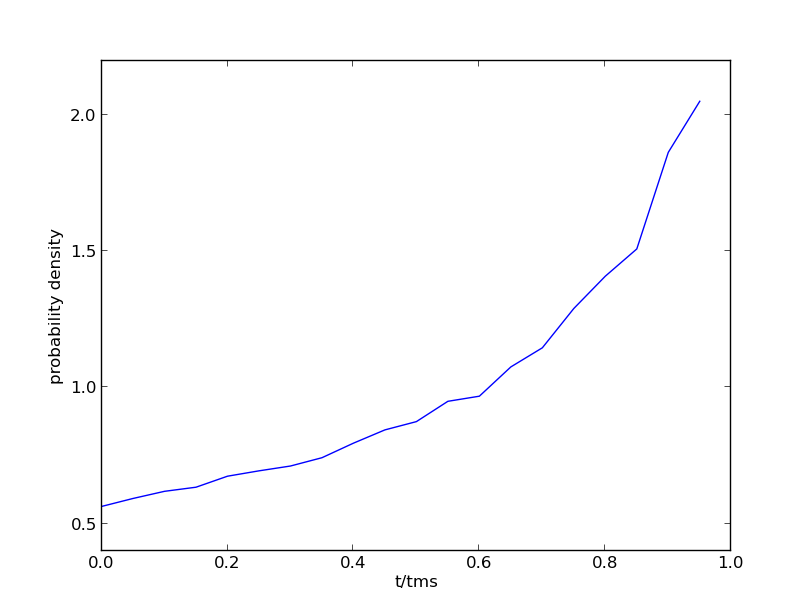
\includegraphics[width=\textwidth]{10-100-100}
  \end{minipage}
  \begin{minipage}{0.49\textwidth}
   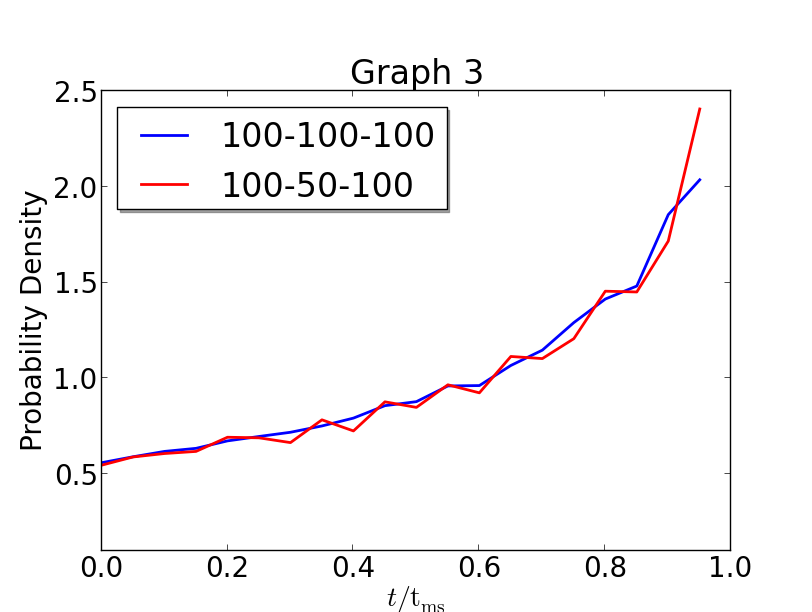
\includegraphics[width=\textwidth]{100-50-100}
  \end{minipage}
  \begin{minipage}{0.49\textwidth}
   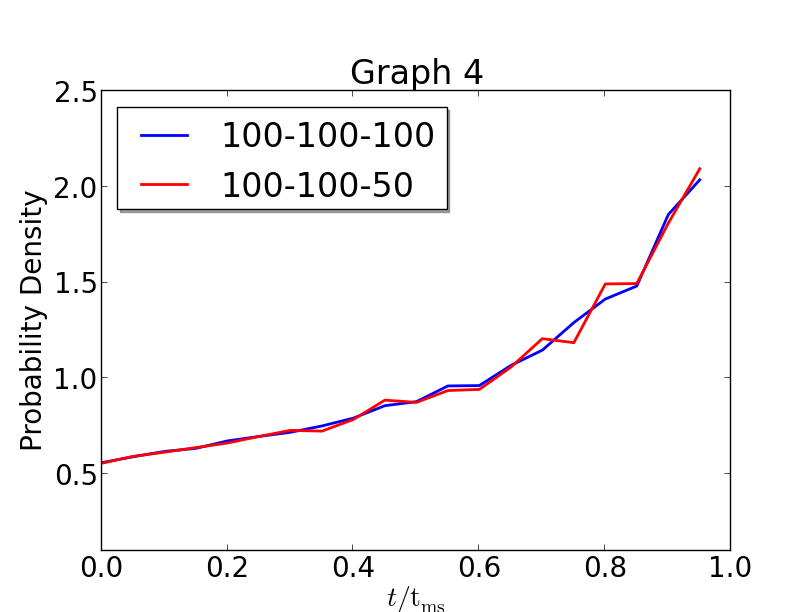
\includegraphics[width=\textwidth]{100-100-50}
  \end{minipage}
   \caption{Probability density function for all stars in my sample with a magnitude cut at V=9 with binnings of 100-100-100 (top left) 
   10-100-100 (top right) 100-50-100 (bottom left) and 100-100-50 (bottom right) in distance-mass-age.\label{binnings}}   
 \end{figure}
 
  Figure \ref{binnings} shows the probability density function for all stars in the sample
  with a magnitude cut at V=9 with different distance-mass-age binnings. The top left graph shows the reference graph
  with a binning of 100 for all variables. For the graph on the top right I reduced the binning in distance by a factor of ten. Both graphs
  are very similar. This means, that distance will be very robust to low binnings. \\
  The bottom two show the same function with the binning in mass (left) and age (right) halved. Here the discrepancies are very obvious. 
  Because of this I use a binning of 100-1000-1000 for my final data.
 
 \newpage
 \section{Results}
 \begin{figure}[h!]
   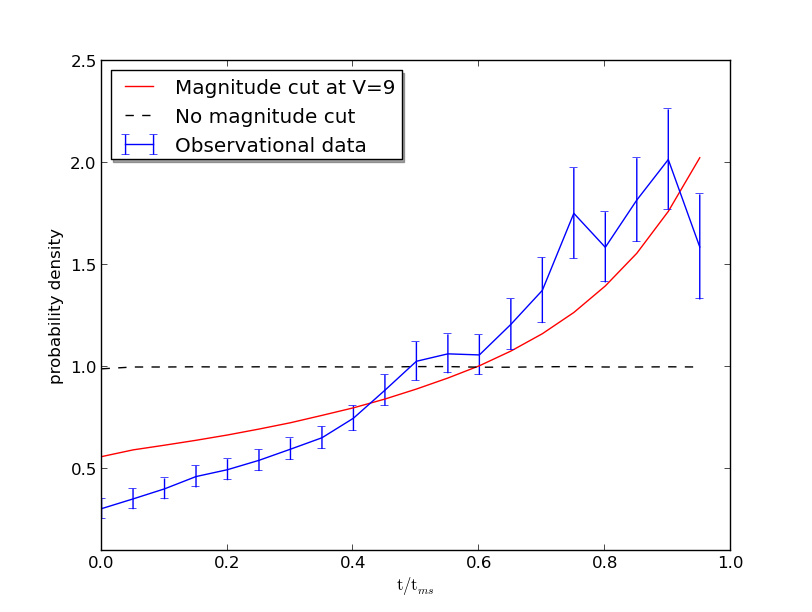
\includegraphics[width=\textwidth]{plot1}
   \caption{Probability density function with magnitude cut at V=9 (red line), probability density function without magnitude cut
   (black line) and observational data with error bars (blue line). All computed Data is obtained using a binning of 100-1000-1000
   in distance-mass-age. The observational data is taken from \textbf{citation?}\label{all3}}
 \end{figure}
 
 Figure \ref{all3} shows the probability density function with magnitude cut at V=9 (red line), probability density function without 
 magnitude cut (black line) and observational data with error bars (blue line).\\
 The probability density function without a magnitude cut shows, that the stars are uniformly distributed in $\tau$.\\
 The blue line seems to have a higher slope, than the red line. They do however compare pretty well 
 considering the program is only a minimalistic model. There are a lot of things, that can still be implemented:\\
 \begin{itemize}
  \item Right now the stars are distributed homogenously in a sphere of a 3kpc radius. To make it more accurate one could model our
  galactic neighborhood. Namely take into account the thickness of the galactic disk, which is smaller, than 3kpc.
  \item The program does not take into account binary stars. 
  \item From observations we know, that we live in a part of the galaxy with little star formation.  
  The density of young open starclusters increases the farther you move away from the solar system. As seen in Figure \ref{clusters}.
  \item My model for reddening is very approximated. It does not take into account density fluctuations in the interstellar medium. 
  The effects of which can be seen in figures \textbf{reference to diffmag}.
 \end{itemize}
 \begin{figure}[h!]
  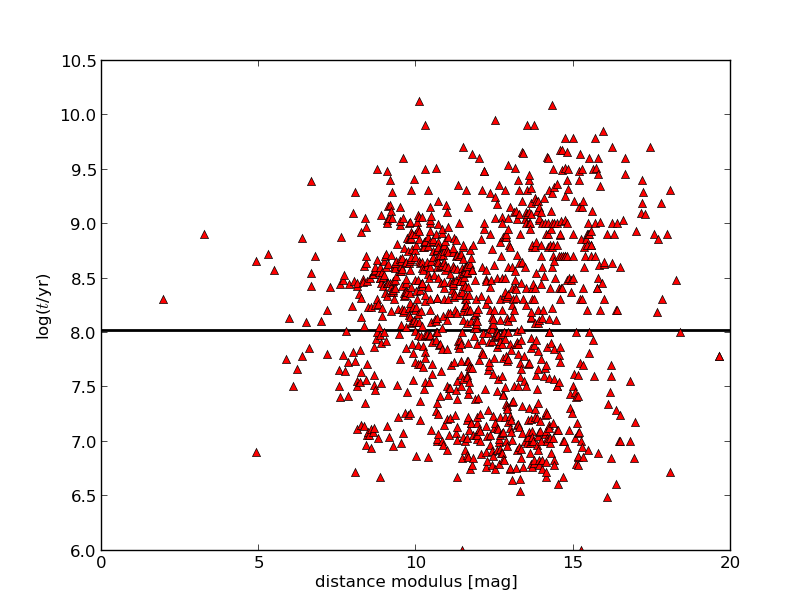
\includegraphics[width=\textwidth]{clusters}
  \caption{Open starclusters in our galaxy with distance modulus vs log(Age/yr)  \label{clusters}}
 \end{figure}

 
 \section{Conclusions}
 
 
 
 \bibliography{adssample}
\end{document}
